
\begin{figure}[h!]
\centering
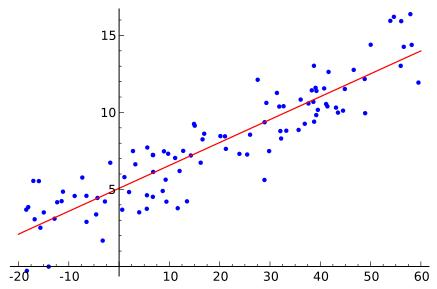
\includegraphics[width=10cm]{images/linear_regression.jpg}
\caption{Ejemplo de Regresión Lineal}
\end{figure}

\section{Análisis de regresión}

Llegado a este punto, dada una variable acústico-prosódica, nos interesó evaluar la relación entre el entrainment y las distintas variables sociales. Con esto en mente, planteamos un modelo de regresión lineal tomando como nuestra variable \emph{explicativa} la mimetización o \entrainment, y la variable \emph{dependiente} será la variable social elegida. Este análisis de regresión nos permitió observar cuál es la variación conjunta de ellas.

Nuestra hipotesis consistió en que la mimetización (por ejemplo, en la intensidad o pitch) se relacionaría de manera directa con ciertas variables sociales de connotación positiva (por ejemplo, la compenetración en el juego) y que se relacionaría de manera inversa con aquellas de carácter negativo (el aburrimiento o el desagrado por su compañero).


\subsection{Modelo clásico de Regresión Lineal}

En el modelo clásico de regresión lineal, tenemos un conjunto de valores fijos $X_1, X_2, \ldots, X_n$, que son llamadas variables independientes. Asociado a cada uno de estos valores fijos, tenemos variables aleatorias $Y_1, \ldots, Y_n$. Asumimos, además, que nuestras variables son de la forma

\begin{equation}
  Y_i = E[Y|X_i] + u_i
\end{equation}

donde $u_i$ es la perturbación estocástica de la variable.

Asumiendo que $E[Y|X_i]$ es una función lineal de $X_i$; es decir, que existen $\beta_1, \beta_2 \in \mathbb{R}$ que cumplen

\begin{equation}
  E[Y|X_i] = \beta_1 + \beta_2 X_i
\end{equation}

obtenemos que

\begin{equation}
  Y_i = \beta_1 + \beta_2 X_i + u_i
\end{equation}

Nuestro objetivo es poder entonces conseguir estimadores $\widehat{\beta_1}, \widehat{\beta_2}$ que nos permitan analizar y predecir el comportamiento conjunto de estas variables.

En la siguiente sección se describe el primer experimento, en el cual utilizamos el modelo ``pooled'' o agrupado, en el cual utilizamos todos los datos juntos indistintamente de la sesión y hablante del que provengan.






